\section{Temperature sweeps}

Figure~\ref{Fig:ExpH:TSweeps} shows the in-plane resistivity, $\rho(T)$ for each of the samples in zero field taken in the \ac{VTI} in the Polo magnet. From this plot we can characterise the \Tc of the samples and find the residual resistivity, $\rho_0$ by using simple linear fits to the data above the transition temperatures and extrapolate back to zero. Table~\ref{Tab:ExpH:TSweeps} show the fit parameters for each of the samples. 
\begin{table}
	\begin{center}
       	\caption{Fits parameters to $\rho = \rho_0 + \rho_1T$ for zero field resistivity data above $T_c$ as well as $T_c$ values determined from the same plots. Fits at low $T$ are shown in inset to figure~\ref{Fig:ExpH:TSweeps}.}
		{\small \begin{tabular}[htbp]{lrrrr}
\toprule
Sample		& $\rho_0 (\unit{\micro\ohm\centi\metre})$	& $\rho_1 (\unit{\micro\ohm\centi\metre})$  & $T_c$ (\unit{\kelvin})	& $T_c/T_c(\textrm{max})$	\\
\midrule
B00KOD1A	& 40.7		& 0.454     & $0\pm1.0$	    & $0.00\pm0.03$	\\
B07KOD2		& 73.0		& 1.026     & $11\pm3.8$	& $0.31\pm0.11$	\\
B16KOD1A	& 49.9		& 0.843     & $17\pm1.0$	& $0.47\pm0.03$	\\
B30KOD3		& 15.9		& 0.578     & $29\pm0.5$	& $0.81\pm0.01$	\\
B32KOP1		& 54.2		& 0.824     & $36\pm1.0$	& $1.00\pm0.03$	\\
B32KOP4		& 55.6		& 1.904     & $35\pm2.0$	& $0.97\pm0.06$	\\
B30KUD3		& 123.0		& 2.233     & $32\pm1.0$	& $0.89\pm0.03$ \\
B28KUD3A	& 22.6		& 0.806     & $32\pm1.0$	& $0.89\pm0.03$	\\
\bottomrule
		\label{Table:ExpH:TSweepFitsParams}
		\end{tabular} }
	\end{center}
\end{table}
The residual resistivities are very good with only one being above \unit{100}{\micro\ohm\centi\metre} and most below \unit{70}{\micro\ohm\centi\metre} which has been cited as being exceptionally good for \ac{BSCO}~\cite{Ando1999}. Moreover the \Tc of the optimally doped sample is \unit{36}{\kelvin} which is amongst the highest reported~\cite{Ando1999} which again is testament to the crystal quality. $\rho_0$ generally increases as you move away from critical doping which lends support to the notion of the La doping increasing the disorder.


% \begin{table}
% 	\begin{center}
%        	\caption{Fits parameters to $\rho = \rho_0 + \alpha_1T + \alpha_2T^2$ for zero field resistivity data above $T_c$. Fits at low $T$ are shown in inset to figure~\ref{Fig:ExpH:TSweeps}}
% 		\begin{tabular}[htbp]{lrrr}
% \toprule
% Sample		& $\rho_0 (\times10^-2)$	& $\alpha_1 (\times10^{-4})$	& $\alpha_2 (\times10^{-7})$	\\
% \midrule
% B00KOD1A	& 12.26		& 6.895		& 14.394		\\
% B07KOD2		& 9.03		& 7.740		& 8.459			\\
% B16KOD1a	& 4.25		& 4.809		& 3.610			\\
% B30KOD3		& 1.43		& 3.385		& 4.595			\\
% B32KOP1		& 1.20		& 2.596		& -0.810		\\
% B32KOP4		& 2.76		& 21.886	& -8.862		\\
% B30KUD3		& 18.80		& 38.028	& -4.385		\\
% B28KUD3a	& 2.71		& 18.447	& -6.756		\\
% \bottomrule
% 		\label{Table:ExpH:TSweepFitsParams}
% 		\end{tabular}
% 	\end{center}
% \end{table}


\section{Field sweeps}

Figures~\ref{Fig:ExpH:HallIndividualOD}, \ref{Fig:ExpH:HallIndividualOP} and \ref{Fig:ExpH:HallIndividualUD} show the Hall coefficients extracted as described in the methods section for samples progressing from overdoped, optimally doped to underdoped respectively. Where appropriate, the data is compared to that from Ando \etal~\cite{Ando1999}. For the samples of $T_C >= \unit{28}{\kelvin}$ there are some data which did not reach sufficient field to obtain linear behaviour which are circled with a dashed line in the plots. Examples of data where the temperature control was poor are also circled.

For sample B30KOD2, many of the sweeps for $T < \unit{45}{\celsius}$ showed significant hysteresis due to temperature drift. Despite temperature correction, many of the fits did not pass through the origin (circled in the figure). The same goes for the circled points in B30KUD2 which also features another data point at \unit{1.5}{\kelvin} from the first trip to \ac{LNCMI} which is outside the plot boundary at \unit{$7.3\times10^{-3}$}{\centi\metre\cubed} and also for data points for B28KUd3b. These points have not been included in the final plots.

The error bars on the data points do not include error from the thicknesses which are large and systematic across the data points. The inset of figure~\ref{Fig:ExpH:InvHallCombined} shows the $R_H$ values at \unit{300}{\kelvin} vs. doping for each of the samples with these error bars applied. The overall trend is downward with doping although the data points are not monotonically decreasing unless we consider the error bars. Since these are large and systematic (i.e. all points in the set will have the same offset) we adjust the data within the errors systematically for the samples B30KUD3, B32KOP1 and B07KOD2 by $\times1.07$, $\times0.91$ and $\times0.89$ respectively so that the data follow the monotonic downward trend. Of course, care should be taken to bear these adjustments in mind when making quantitative statements about the trends in doping. The adjusted data sets are shown in the main panels of figure~\ref{Fig:ExpH:InvHallCombined} alongside the data from the Ando paper.

\begin{figure}[htbp]
	\begin{center}
		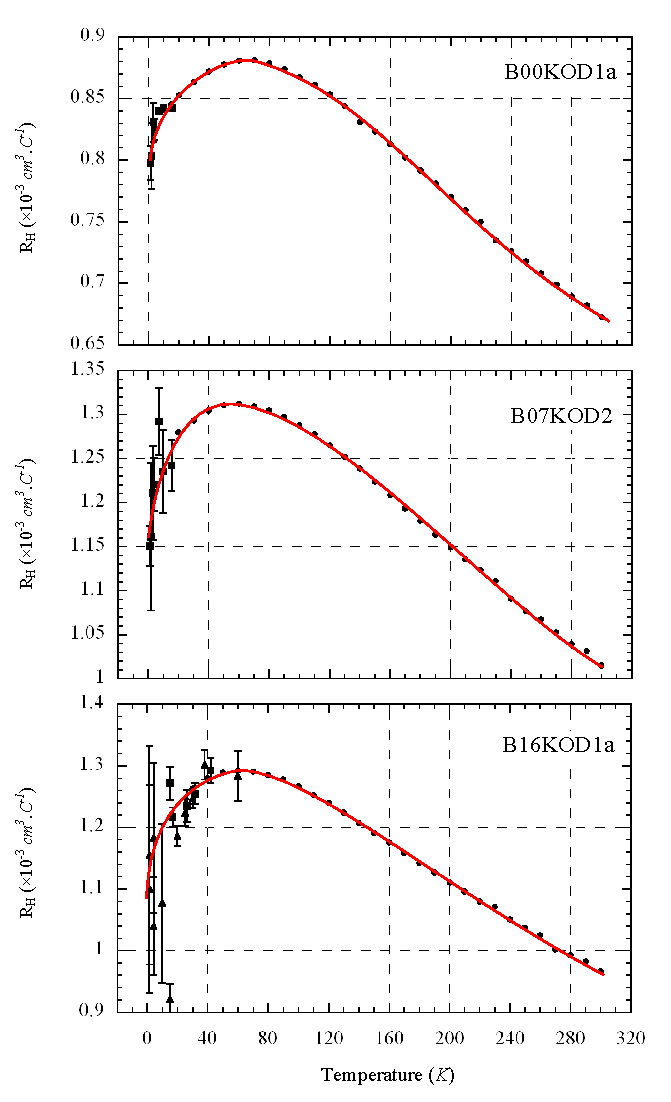
\includegraphics[scale=0.9]{Chapter-HallBSCO/Figures/HallIndividual/HallIndividualOD}
		\caption{$R_H$ for underdoped samples of \ac{BSCO}. Plots show results from, $\bullet$ Polo in June 2010, $\blacktriangle$ \ac{LNCMI} in June 2009, $\blacktriangledown$ \ac{LNCMI} in Feb 2010, $\blacksquare$ Nijmegen in May 2010. Symbols for comparable samples are marked on the plots. Red lines are a guide to the eye.}
		\label{Fig:ExpH:HallIndividualOD}
	\end{center}
\end{figure}

\begin{figure}[htbp]
	\begin{center}
		\includegraphics[scale=0.9]{Chapter-HallBSCO/Figures/HallIndividual/HallIndividualOP}
		\caption{$R_H$ for underdoped samples of \ac{BSCO}. Plots show results from, $\bullet$ Polo in June 2010, $\blacktriangle$ \ac{LNCMI} in June 2009, $\blacktriangledown$ \ac{LNCMI} in Feb 2010, $\blacksquare$ Nijmegen in May 2010. Symbols for comparable samples are marked on the plots. Dashed lines indicate points where the field was not sufficient to achieve linear behaviour. Red lines are a guide to the eye.}
		\label{Fig:ExpH:HallIndividualOP}
	\end{center}
\end{figure}

\begin{figure}[htbp]
	\begin{center}
		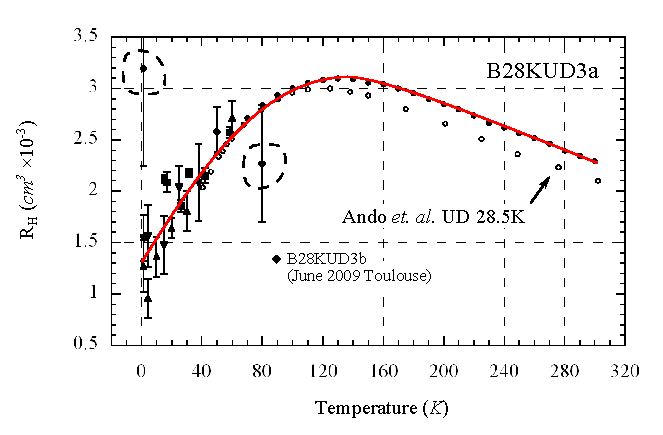
\includegraphics[scale=0.9]{Chapter-HallBSCO/Figures/HallIndividual/HallIndividualUD}
		\caption{$R_H$ for underdoped samples of \ac{BSCO}. Plots show results from, $\bullet$ Polo in June 2010, $\blacktriangle$ \ac{LNCMI} in June 2009, $\blacktriangledown$ \ac{LNCMI} in Feb 2010, $\blacksquare$ Nijmegen in May 2010. Symbols for comparable samples are marked on the plots. Dashed lines indicate points where the field was not sufficient to achieve linear behaviour. Red lines are a guide to the eye.}
		\label{Fig:ExpH:HallIndividualUD}
	\end{center}
\end{figure}
\begin{figure}[htbp]
	\begin{center}
		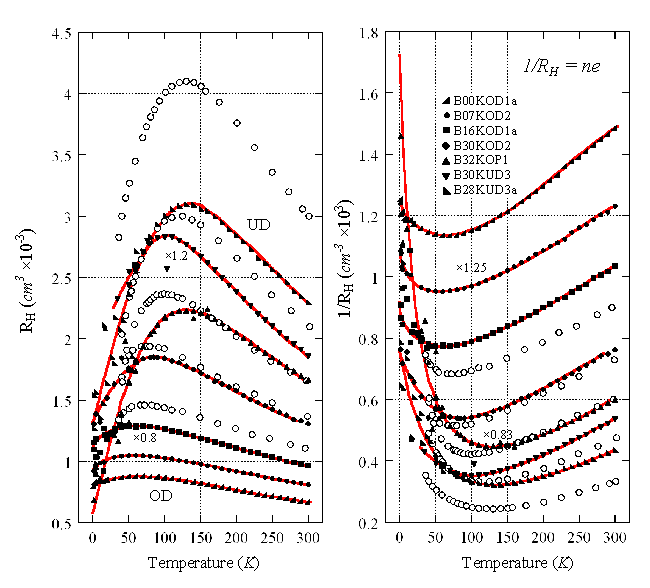
\includegraphics[scale=1.1]{Chapter-HallBSCO/Figures/InvHallCombined/InvHallCombined}
		\caption{Hall data in context with data from Ando \etal\cite{Ando1999} (open circles) which are in order of increasing $R_H$, 24KOD, 30KOD, 33KOP, 28.5KUD, 20KUD. Right panel shows the inverse hall data which relates to carrier density. Red lines are the same guides to the eye used in previous figures. Inset shows $R_H$ at \unit{300}{\kelvin} plus systematic error bars due primarily to uncertainty in thickness vs. doping scaled to \ac{TL2201} data. B30KUD3 (circled) is plotted in both the overdoped and underdoped positions.}
		\label{Fig:ExpH:InvHallCombined}
	\end{center}
\end{figure}

With reference to figure~\ref{Fig:ExpH:InvHallCombined} and in particular the new low temperature data points, we see that doping strongly affects the qualitative shape of the $R_H$ curves. Whilst the trend appears to be that $R_H(\unit{300}{\kelvin})$ decreases as doping increases as to be expected, the $R_H(\unit{0}{\kelvin})$ values all tend toward approximately similar values of around \unit{$0.5\times 10^{-3}$}{\centi\metre\cubed}to \unit{$1.5\times 10^{-3}$}{\centi\metre\cubed}. The most pronounced difference between high and low temperature values though is with the optimally doped samples which are around $\times 2.75$ greater at high temperature.

Right down to \unit{0}{\kelvin} there is no sign change in $R_H$, which confirms that the hole pockets have higher mobility than the electron pockets across the range of dopings studied.

\begin{figure}[htbp]
    \begin{center}
        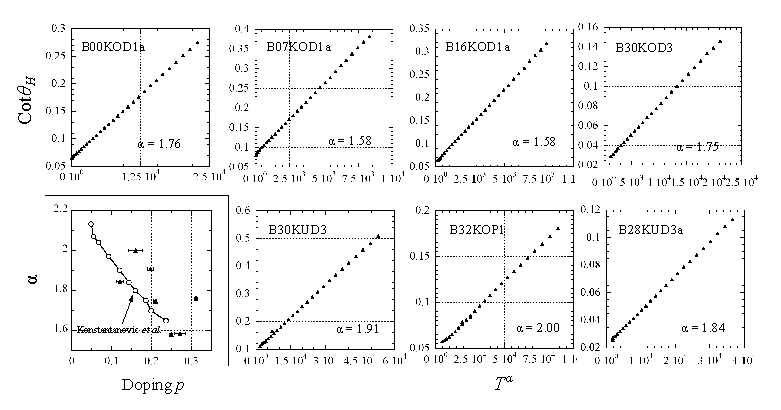
\includegraphics[scale=1.0]{Chapter-HallBSCO/Figures/HallAngle/HallAngle}
        \caption{Hall angle calculated with a nominal field of unity. Fitted powers are labelled.}
        \label{Fig:ExpH:HallAngle}
    \end{center}
\end{figure}



There seems to be little evidence of the transition of the doping from $p$ to $1+p$ which agrees with the notion that these dopings lie beyond where the Fermi surface reconstruction is thought to take place~\cite{LeBoeuf2007}. 

\begin{figure}[htbp]
    \begin{center}
        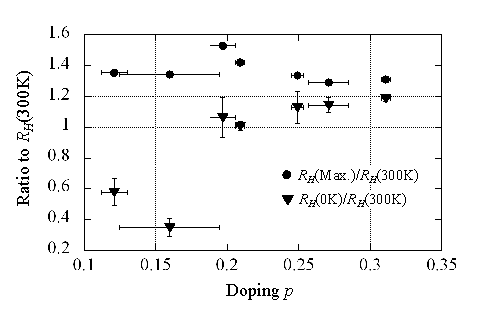
\includegraphics[scale=0.9]{Chapter-HallBSCO/Figures/RhRatios/RhRatios}
        \caption{Ratio of $R_H$ values at the maximum of the Hall curves and at $T=\unit{0}{\kelvin}$ to the $T=\unit{300}{\kelvin}$ $R_H$ values. Errors in $R_H(\unit{0}{\kelvin}$ estimated from Hall plots, the value for B30KUD2 is estimated based on linear extrapolation.}
        \label{Fig:ExpH:RhRatios}
    \end{center}
\end{figure}
%Divergence in resistivity occurs beyond UD 0K\cite{Ando2000}, well
%below our lowest nominal doping of ...

% Residual resistivity of ~20\mu\Ohm cm at optimal doping is very small
% and increases with La doping i.e. as become more underdoped
% \cite{Ando2000}


